\chapter{Introduction}
\label{chapter:introduction}

\section{Background}
Road accidents remain a global public health crisis, with the World Health Organization estimating over 1.3 million deaths annually due to traffic collisions. Overspeeding has been identified as one of the primary contributing factors in these incidents, significantly increasing both the likelihood of accidents and their severity when they occur. In many jurisdictions, speed limits are set as static values based on road type and local regulations, often without accounting for real-time environmental conditions that directly affect braking distance and driver reaction time.

Factors such as weather conditions, visibility, time of day, and location type play critical roles in determining safe driving speeds. For instance, a speed limit of 60 km/h that is appropriate for clear weather and daylight conditions becomes dangerously excessive during heavy rain, fog, or nighttime. Traditional static speed limit systems fail to account for these dynamic variables, leaving drivers without adequate guidance for adapting their speed to current road conditions.

\section{Problem Statement}
Current speed limit systems rely on fixed values that do not adapt to changing environmental conditions. This creates a significant safety gap, particularly when drivers encounter sudden changes in weather, visibility, or road circumstances. The absence of personalized, context-aware speed recommendations means that drivers must manually assess conditions and make speed decisions without systematic support. This disconnect between static regulations and real-world driving conditions contributes to preventable accidents, especially during adverse weather events, low-light situations, or in high-risk zones such as school areas and construction zones.

Existing solutions often require manual input from drivers for various parameters, or they lack integration of multiple data sources that could provide comprehensive risk assessment. There is a need for an intelligent system that automatically detects environmental factors and provides dynamic speed recommendations tailored to current conditions.

\section{Motivation for Dynamic Speed Systems}
The emergence of mobile technology, GPS capabilities, and real-time data processing creates opportunities for more intelligent driving assistance systems. Dynamic speed systems address the limitations of static speed limits by continuously monitoring environmental conditions and adjusting speed recommendations accordingly. These systems leverage multiple data sources—including GPS location, camera-based visibility detection, weather information, and time-of-day assessments—to generate contextually appropriate speed guidance.

The motivation behind this research is to develop a practical solution that bridges the gap between regulatory speed limits and real-world driving conditions. By providing drivers with personalized, real-time speed recommendations, we aim to reduce accidents caused by inappropriate speeds while maintaining the flexibility needed for safe navigation across varying conditions.

\section{Overview of the Dynamic Speed Limit System}
This project presents the Dynamic Speed Limit System (DSLS), a Flutter-based Android application that calculates and displays recommended driving speeds based on real-time environmental conditions. The system integrates multiple data sources to provide comprehensive speed recommendations:

\begin{itemize}
    \item \textbf{GPS Tracking}: Real-time vehicle speed monitoring using GPS data with fallback distance/time calculations
    \item \textbf{Weather Integration}: User-configurable weather conditions including clear, cloudy, rain, heavy rain, fog, snow, and storm
    \item \textbf{Time of Day Assessment}: Automatic detection of time periods (morning, afternoon, evening, night) from device clock
    \item \textbf{Location Type Inference}: Automatic inference of location type (urban, suburban, highway, residential, school zone, construction zone) based on GPS speed
    \item \textbf{Visibility Detection}: Camera-based ambient light detection to assess visibility conditions
\end{itemize}

The DSLS employs a multiplicative factor algorithm that combines weather, time, location, and visibility parameters to calculate recommended speeds. A risk engine evaluates these factors to generate a risk score (0-100\%) categorized as low (0-40\%), medium (40-70\%), or high (70-100\%) danger levels.

The user interface provides a visual speedometer with color-coded safety indicators (green, yellow, red) that alert drivers to safe, cautious, or dangerous speed conditions relative to their current environment.

\section{Project Objectives}
\subsection{Main Objective}
To develop a Flutter-based mobile application that provides dynamic speed recommendations based on real-time environmental conditions, thereby enhancing road safety by guiding drivers to adapt their speeds appropriately.

\subsection{Specific Objectives}
\begin{enumerate}[(i)]
    \item To develop a GPS-based speed tracking system for real-time vehicle monitoring
    \item To implement automatic detection of environmental parameters including weather, visibility, time of day, and location type
    \item To design and implement a risk assessment engine that evaluates multiple factors to generate speed recommendations
    \item To develop a user-friendly interface with visual feedback on safe driving speeds
\end{enumerate}

\section{Research Questions}
\begin{enumerate}[(i)]
    \item How can real-time environmental data be effectively integrated to generate accurate speed recommendations?
    \item What is the optimal algorithm for combining multiple risk factors into a cohesive speed recommendation system?
    \item How can the system balance accuracy with user convenience in parameter detection?
    \item How effectively does the system respond to changing environmental conditions?
\end{enumerate}

\section{Project Significance}
\subsection{Value Proposition}
The DSLS provides immediate value to drivers by offering personalized, context-aware speed guidance that static speed limits cannot provide. The system empowers drivers to make safer decisions based on current conditions rather than relying solely on fixed regulatory limits.

\subsection{Innovation}
The system innovatively combines multiple automatic detection methods—GPS speed tracking, camera-based visibility assessment, and device time analysis—into a cohesive platform that requires minimal user input while providing comprehensive recommendations.

\subsection{Impact}
By reducing speed-related accidents through intelligent speed guidance, the DSLS has the potential to save lives and reduce the economic burden of road accidents on healthcare and insurance systems.

\section{Scope of the Study}
This study focuses on the development and evaluation of the Dynamic Speed Limit System as an Android mobile application. The research covers system design, implementation of core services (GPS tracking, visibility detection, auto parameters), risk calculation algorithms, and user interface development. Future enhancements such as live weather API integration, map-based location detection, and speed limit database integration are identified but fall outside the current scope.
%\newpage

%%%%%%%%%%%%%%%%%%%%%%%%%%%%% Literature Review Section%%%%%%%%%%%%%%%%%%%%%%%%%%%%%%%%%%%%%%
\chapter{Literature Review}\label{chapter:Literature_Review}
\section{Literature Review}
In this section, we present the findings from several literature sources with regard to the major concepts associated with this research. Information obtained from several journal articles, conference papers, relevant workshops, reputable websites, and published books are compiled to provide theoretical grounding and practical justification for the problem under investigation.
\section{Intelligent Transport Systems}
Intelligent Transport Systems (ITS) represent a broad category of technology applications designed to improve transportation safety, efficiency, and sustainability through the integration of information and communication technologies. According to the European Union's ITS Directive, ITS encompasses systems where information and communication technologies are applied in the field of road transport, including infrastructure, vehicles, and users, as well as traffic management and mobility management. The literature demonstrates that ITS has evolved significantly over the past two decades, progressing from basic traffic monitoring systems to sophisticated autonomous driving assistance platforms.

Research by Khan et al. (2021) highlights the role of ITS in reducing road accidents through real-time traffic management and driver assistance features. Modern ITS applications incorporate vehicle-to-infrastructure (V2I) and vehicle-to-vehicle (V2V) communication protocols that enable continuous data exchange between vehicles and roadside systems. These developments have paved the way for more advanced speed management systems that can respond to dynamic environmental conditions rather than relying solely on pre-programmed speed limits.

The Dynamic Speed Limit System (DSLS) presented in this research aligns with ITS principles by leveraging multiple data sources—including GPS tracking, camera-based visibility detection, and weather data—to provide context-aware speed recommendations. Unlike traditional ITS implementations that focus primarily on traffic flow optimization, DSLS prioritizes individual driver safety by personalizing speed guidance based on real-time environmental factors.

\section{GPS-Based Vehicle Tracking}
Global Positioning System (GPS) technology has become ubiquitous in modern vehicle navigation and tracking applications. The literature extensively documents the use of GPS for vehicle speed monitoring, route tracking, and fleet management. According to Taylor et al. (2020), GPS-based speed measurement offers advantages over traditional speedometer readings due to its accuracy in measuring ground speed independent of wheel slip or tire wear.

However, existing GPS-based systems primarily focus on navigation and location tracking rather than safety applications. Chen and Zhang (2019) note that while GPS technology is widely available in smartphones and dedicated navigation devices, its potential for enhancing driver safety through speed recommendations remains underutilized. Most existing applications use GPS solely for displaying current speed without considering environmental factors that affect safe driving speeds.

The DSLS extends GPS-based tracking beyond simple speed display by integrating GPS data with other environmental parameters. The system uses GPS speed to not only show current vehicle speed but also to infer location type (urban, suburban, highway) based on typical speed ranges. This approach represents an advancement over existing GPS applications that treat speed as a standalone metric without contextual interpretation.

\section{Environmental Data Integration in Driving Systems}
The integration of environmental data—including weather conditions, visibility, and time of day—into driving assistance systems has gained attention in recent research. Studies by Wang et al. (2022) demonstrate that weather conditions significantly impact braking distance and driver reaction times, with rain reducing visibility by up to 50\% and increasing stopping distances by 30-40\% compared to dry conditions. Similarly, research by Brown et al. (2021) shows that fog conditions can reduce visibility to less than 100 meters, requiring significant speed reductions to maintain safe stopping distances.

Visibility detection using camera-based sensors has been explored in academic literature. Li and Park (2020) propose using smartphone camera sensors to detect ambient light levels and assess visibility conditions for driver assistance applications. Their research demonstrates the feasibility of using built-in camera hardware for environmental monitoring without requiring additional specialized sensors.

Time-of-day considerations have also been addressed in the context of driving safety. Statistics from the National Highway Traffic Safety Administration indicate that fatal accident rates are significantly higher during nighttime hours, with the period between 6 PM and 6 AM accounting for a disproportionate share of traffic fatalities. This research highlights the need for speed recommendation systems that account for reduced visibility and driver fatigue during evening and night hours.

The DSLS integrates all these environmental factors—weather, visibility via camera, and time of day—into a cohesive risk assessment framework. Unlike existing systems that address these factors in isolation, DSLS combines multiple parameters using a multiplicative factor algorithm to generate comprehensive speed recommendations.

\section{Limitations of Static Speed Limit Systems in Navigation Platforms}
Existing navigation platforms, including Google Maps, Waze, and Apple Maps, provide speed limit information as static values associated with specific road segments. While these systems offer valuable guidance for drivers, they suffer from fundamental limitations that prevent them from addressing real-time driving conditions. Research by Martinez et al. (2021) identifies several critical shortcomings of static speed limit approaches.

First, static speed limits do not account for weather conditions. A speed limit of 60 km/h posted for dry conditions becomes inappropriate during heavy rain, snow, or fog, yet navigation systems provide no adjustment for these environmental factors. Second, static systems cannot account for visibility changes throughout the day, failing to recommend reduced speeds during periods of low light or glare. Third, these platforms cannot detect special zones such as school zones or construction areas that may have variable speed requirements based on time of day or activity.

Google Maps and similar platforms rely on mapping databases that store speed limit information as fixed attributes of road segments. According to Thompson et al. (2022), updating these databases requires significant manual effort and cannot respond to temporary conditions such as road work, school zone activity, or adverse weather. This static approach creates a gap between regulatory speed limits and conditions-appropriate safe speeds.

The DSLS addresses these limitations by providing dynamic speed recommendations that adapt to current environmental conditions rather than relying on fixed database values. By integrating real-time data from multiple sources, DSLS offers a significant advancement over static navigation approaches.

\section{Risk Assessment Models in Transportation Safety}
Transportation safety research has developed various risk assessment models to quantify the danger associated with different driving conditions. The traffic conflict technique (TCT) proposed by Hyden (1987) remains influential, using observed vehicle interactions to assess safety levels. More recent approaches incorporate multiple risk factors into composite indices that account for environmental, vehicular, and human factors.

Research by Elvik et al. (2019) demonstrates that speed is among the most significant factors influencing accident severity, with a nonlinear relationship between speed and crash risk. Their meta-analysis shows that reducing mean speed by 1 km/h can reduce crash rates by 2-4\% depending on the road type. This research supports the rationale for dynamic speed systems that encourage drivers to adjust speeds based on conditions.

The DSLS implements a risk assessment engine that calculates a risk score (0-100\%) based on four key parameters: weather, time of day, location type, and visibility. The risk score is categorized as low (0-40\%), medium (40-70\%), or high (70-100\%) to provide drivers with clear feedback on current driving conditions. This approach aligns with established risk assessment principles while providing practical, actionable guidance.

\section{Summary and Research Gap}
The literature review reveals that while significant research has been conducted in intelligent transport systems, GPS tracking, environmental data integration, and risk assessment, there remains a gap in systems that dynamically combine multiple environmental factors to generate personalized speed recommendations. Existing navigation platforms provide static speed limits that do not adapt to changing conditions, while driving assistance systems often address environmental factors in isolation.

This research addresses the identified gap by developing the Dynamic Speed Limit System (DSLS), which integrates GPS tracking, weather conditions, time of day, location type inference, and camera-based visibility detection into a cohesive platform. The system represents an advancement over existing approaches by providing comprehensive, real-time speed recommendations that account for multiple environmental factors simultaneously.

\chapter{Methodology}\label{chapter:Methodology}
\section{System Approach}
The Dynamic Speed Limit System (DSLS) employs a rule-based dynamic approach that integrates real-time environmental data to generate personalized speed recommendations. Unlike static speed limit systems that rely on fixed database values, DSLS continuously monitors multiple environmental parameters and calculates safe speeds based on their current values. The system operates on a multiplicative factor model where each environmental condition contributes a normalized factor (0-1) to the overall risk calculation. These factors are combined to produce a risk score that directly influences the recommended driving speed.

The methodology follows a data-driven approach where input parameters are acquired from various sensors and services, processed through a risk calculation engine, and output as speed recommendations displayed on the user interface. This approach ensures that recommendations reflect actual driving conditions rather than theoretical or historical values.

\section{Data Acquisition}
The system acquires data from four primary sources, each providing critical information for risk assessment:

\subsection{GPS Speed and Location Service}
The GPS Speed Service (\texttt{gps\_speed\_service.dart}) provides real-time vehicle speed tracking using GPS data. The service monitors GPS signal status and provides speed updates in real-time. In cases where GPS speed data is unavailable (such as poor signal conditions), the service falls back to calculating speed based on distance traveled over time. The service also infers location type based on GPS speed readings: speeds below 30 km/h indicate urban areas, speeds between 30-70 km/h indicate suburban zones, and speeds above 70 km/h indicate highway conditions.

\subsection{Weather Data}
Weather conditions are input through user configuration, with options for clear, cloudy, rain, heavy rain, fog, snow, and storm conditions. Each weather condition carries a predefined multiplier that reflects its impact on safe driving speeds. In future implementations, the system will integrate with weather APIs to automatically fetch current conditions based on GPS location.

\subsection{System Time}
The Auto Parameters Service (\texttt{auto\_parameters\_service.dart}) automatically detects time of day from the device clock. Time periods are categorized as morning (5 AM - 12 PM), afternoon (12 PM - 5 PM), evening (5 PM - 8 PM), and night (8 PM - 5 AM). Each time period carries a multiplier reflecting typical visibility and traffic conditions: afternoon receives full multiplier (100\%) while night receives the lowest (60\%).

\subsection{Simulation Inputs}
The system includes a simulation feature that allows manual override of all parameters for testing purposes. Users can input custom values for weather, time, location, and visibility to test how different scenarios affect recommended speeds. This feature enables thorough testing of the risk calculation model without requiring actual environmental conditions.

\section{Risk Calculation Model}
The risk calculation model normalizes each input parameter to a 0-1 scale and combines them to produce an overall risk factor. The normalization ensures that parameters with different scales (such as weather conditions versus location types) are properly weighted in the final calculation.

\subsection{Normalization Process}
Each parameter is mapped to a normalized value representing its contribution to safe driving:

\begin{table}[h]
\centering
\caption{Weather Factor Normalization}
\label{tab:weather}
\begin{tabular}{|l|c|}
\hline
\textbf{Condition} & \textbf{Factor} \\
\hline
Clear & 1.00 \\
Cloudy & 0.95 \\
Rain & 0.75 \\
Heavy Rain & 0.50 \\
Fog & 0.60 \\
Snow & 0.45 \\
Storm & 0.40 \\
\hline
\end{tabular}
\end{table}

\begin{table}[h]
\centering
\caption{Time of Day Factor Normalization}
\label{tab:time}
\begin{tabular}{|l|c|}
\hline
\textbf{Period} & \textbf{Factor} \\
\hline
Morning (5AM-12PM) & 0.90 \\
Afternoon (12PM-5PM) & 1.00 \\
Evening (5PM-8PM) & 0.75 \\
Night (8PM-5AM) & 0.60 \\
\hline
\end{tabular}
\end{table}

\begin{table}[h]
\centering
\caption{Location Type Factor Normalization}
\label{tab:location}
\begin{tabular}{|l|c|}
\hline
\textbf{Location Type} & \textbf{Factor} \\
\hline
Highway & 1.00 \\
Suburban & 0.85 \\
Urban & 0.70 \\
Residential & 0.50 \\
School Zone & 0.30 \\
Construction Zone & 0.40 \\
\hline
\end{tabular}
\end{table}

\begin{table}[h]
\centering
\caption{Visibility Factor Normalization}
\label{tab:visibility}
\begin{tabular}{|l|c|}
\hline
\textbf{Visibility Level} & \textbf{Factor} \\
\hline
Excellent & 1.00 \\
Good & 0.90 \\
Moderate & 0.75 \\
Poor & 0.55 \\
Very Poor & 0.35 \\
\hline
\end{tabular}
\end{table}

\subsection{Weighted Combination}
The overall safety factor is calculated by multiplying all four normalized factors:

\begin{equation}
\text{Safety Factor} = F_{weather} \times F_{time} \times F_{location} \times F_{visibility}
\end{equation}

The risk factor (R) is then derived as:

\begin{equation}
R = 1 - \text{Safety Factor}
\end{equation}

This multiplicative approach ensures that poor conditions in any category significantly impact the final recommendation, reflecting the real-world compounding effect of adverse conditions on driving safety.

\section{Speed Recommendation Formula}
The recommended speed is calculated using the formula:

\begin{equation}
\text{Recommended Speed} = \text{Base Speed Limit} \times (1 - R)
\end{equation}

Where:
\begin{itemize}
    \item \textit{Base Speed Limit} is the user's configured speed limit (default: 60 km/h)
    \item \textit{R} is the risk factor (0-1), where 0 represents minimum risk and 1 represents maximum risk
\end{itemize}

For example, with a base speed of 60 km/h and conditions of Clear weather (1.00), Afternoon (1.00), Urban (0.70), and Excellent visibility (1.00):
\begin{equation}
\text{Safety Factor} = 1.00 \times 1.00 \times 0.70 \times 1.00 = 0.70
\end{equation}
\begin{equation}
R = 1 - 0.70 = 0.30
\end{equation}
\begin{equation}
\text{Recommended Speed} = 60 \times (1 - 0.30) = 60 \times 0.70 = 42 \text{ km/h}
\end{equation}

\section{Data Flow Through the System}
The data flow through the DSLS follows a sequential pipeline from input acquisition to speed recommendation display:

\begin{enumerate}
    \item \textbf{Step 1 - Data Acquisition}: The GPS Speed Service begins tracking vehicle speed and location. The Auto Parameters Service reads system time and infers location type from GPS speed. The Visibility Service captures ambient light using the camera and maps brightness to visibility levels. Weather data is received from user input or (in future) weather API.
    
    \item \textbf{Step 2 - Parameter Transmission}: Each service transmits its parameters to the Speed Calculator (located in \texttt{speed\_calculator.dart}). The GPS service provides current speed and location type. The Auto Parameters service provides time of day. The Visibility service provides visibility level. Weather is passed directly from user configuration.
    
    \item \textbf{Step 3 - Normalization}: The Speed Calculator normalizes each parameter using the predefined factor tables. For example, if weather is "Rain," the factor is set to 0.75; if time is "Night," the factor is set to 0.60.
    
    \item \textbf{Step 4 - Risk Calculation}: The normalized factors are combined using the multiplicative formula to calculate the overall safety factor. The risk factor R is derived as 1 minus the safety factor.
    
    \item \textbf{Step 5 - Speed Calculation}: The recommended speed is calculated using the formula: base\_speed × (1 - R). This produces a value that adjusts appropriately based on current conditions.
    
    \item \textbf{Step 6 - Display and Feedback}: The Speed Screen displays both current GPS speed and recommended speed. The interface uses color-coded borders (green for safe, yellow for caution, red for dangerous) to provide immediate visual feedback. Risk level indicators show LOW (0-40\% risk), MEDIUM (40-70\% risk), or HIGH (70-100\% risk).
    
    \item \textbf{Step 7 - Continuous Update}: The system continuously repeats this pipeline, updating recommendations every time any input parameter changes, ensuring drivers receive current advice based on evolving conditions.
\end{enumerate}

This data flow ensures that all environmental factors are properly integrated into the speed recommendation, providing drivers with accurate, context-aware guidance that adapts to their specific driving situation.

\chapter{System Design}\label{chapter:SystemDesign}
\section{System Architecture Overview}
The Dynamic Speed Limit System (DSLS) follows a layered architecture that separates concerns across distinct processing layers. This design ensures maintainability, scalability, and clear separation between data acquisition, processing, and presentation. The system consists of six primary layers that work together to transform raw environmental data into actionable speed recommendations.

\subsection{Layered Architecture}
The system architecture comprises the following layers in sequential order:

\begin{enumerate}
    \item \textbf{Data Sources Layer}: Hardware and system inputs including GPS receiver, camera sensor, device clock, and user input interface.
    \item \textbf{Data Acquisition Layer}: Services responsible for capturing and preparing data from sources (gps\_speed\_service.dart, auto\_parameters\_service.dart, visibility\_service.dart).
    \item \textbf{Processing Layer}: Core business logic including the SpeedCalculator model that performs risk calculations.
    \item \textbf{Risk Engine Layer}: Specialized component within the SpeedCalculator that evaluates environmental factors and generates risk scores.
    \item \textbf{Decision Layer}: Determines recommended speeds based on risk calculations and generates warnings.
    \item \textbf{UI Layer}: Presentation layer displaying speed recommendations, risk levels, and warnings to users.
\end{enumerate}

This layered approach ensures that changes in one layer (such as replacing the weather input source) do not affect other layers, providing flexibility for future enhancements.

\section{Module Descriptions}
The system is composed of four primary modules that implement the layered architecture:

\subsection{GPS Speed Service (\texttt{gps\_speed\_service.dart})}
The GPS Speed Service handles real-time vehicle speed tracking using GPS data. It provides the following functionality:
\begin{itemize}
    \item \textbf{Permission Management}: Checks and requests location permissions from the device operating system.
    \item \textbf{Speed Tracking}: Uses GPS speed when available, with automatic fallback to distance/time calculation when GPS speed is unavailable.
    \item \textbf{Signal Monitoring}: Monitors GPS signal health with status indicators (inactive, active, lost).
    \item \textbf{Real-time Updates}: Provides continuous speed updates clamped between 0-300 km/h.
\end{itemize}

The service uses the Geolocator package and emits position updates through a stream, handling errors gracefully and providing fallback calculations when GPS data is unreliable.

\subsection{Auto Parameters Service (\texttt{auto\_parameters\_service.dart})}
The Auto Parameters Service serves as the central data acquisition hub that manages all four key parameters required for speed calculation:

\begin{itemize}
    \item \textbf{Weather}: User-configurable weather conditions (clear, cloudy, rain, heavy rain, fog, snow, storm). Future versions will integrate weather APIs for automatic fetching.
    \item \textbf{Time of Day}: Automatically detected from device clock using the updateTimeOfDay() method (morning: 5AM-12PM, afternoon: 12PM-5PM, evening: 5PM-8PM, night: 8PM-5AM).
    \item \textbf{Location Type}: Inferred from GPS speed readings (urban: $<$30 km/h, suburban: 30-70 km/h, highway: $>$70 km/h).
    \item \textbf{Visibility}: Updated from camera-based visibility detection service.
\end{itemize}

This service acts as the bridge between raw data sources and the processing layer, providing a unified interface for parameter acquisition.

\subsection{Visibility Service (\texttt{visibility\_service.dart})}
The Visibility Service detects ambient visibility conditions using the device camera. It captures ambient light levels and maps them to visibility categories:
\begin{itemize}
    \item \textbf{Excellent}: Brightness $>$ 180
    \item \textbf{Good}: Brightness 100-180
    \item \textbf{Moderate}: Brightness 50-100
    \item \textbf{Poor}: Brightness 20-50
    \item \textbf{Very Poor}: Brightness $<$ 20
\end{itemize}

The service calculates brightness by sampling pixels from camera images and computing average RGB values, providing automatic visibility updates every 5 seconds.

\subsection{Speed Calculator / Risk Engine (\texttt{speed\_calculator.dart})}
The SpeedCalculator model contains the core risk engine that processes all parameters and generates speed recommendations. It includes:

\begin{itemize}
    \item \textbf{Parameter Classes}: SpeedParameters (weather, timeOfDay, location, visibility, baseSpeedLimit) and SpeedCalculationResult (recommendedSpeed, riskLevel, riskDescription, warnings).
    \item \textbf{Multiplier Functions}: Four getter methods that return factor values for each parameter:
        \begin{itemize}
            \item \_getWeatherMultiplier(): Maps WeatherCondition enum to 0-100 factor
            \item \_getTimeMultiplier(): Maps DayPeriod enum to factor
            \item \_getLocationMultiplier(): Maps LocationType enum to factor
            \item \_getVisibilityMultiplier(): Maps VisibilityLevel enum to factor
        \end{itemize}
    \item \textbf{Calculation Method}: The calculate() method combines all factors using the formula: overallMultiplier = (weather + time + location + visibility) / 400, then applies to base speed.
    \item \textbf{Risk Assessment}: Generates risk descriptions (HIGH/MEDIUM/LOW) and warning messages based on current conditions.
\end{itemize}

This module serves as both the processing layer and risk engine, containing all business logic for speed recommendation generation.

\section{Data Flow Diagram}
The data flow through the system follows a sequential pipeline:

\begin{figure}[h]
\centering
\begin{tikzpicture}[node distance=2cm, auto]
\node[block] (gps) {GPS Service\\(gps\_speed\_service)};
\node[block, right of=gps] (auto) {Auto Parameters Service\\(auto\_parameters\_service)};
\node[block, right of=auto] (calc) {Speed Calculator\\(risk engine)};
\node[block, right of=calc] (ui) {Speed Screen\\(UI Layer)};

\draw[->] (gps) -- node {speed} (auto);
\draw[->] (auto) -- node {parameters} (calc);
\draw[->] (calc) -- node {recommendation} (ui);
\end{tikzpicture}
\caption{System Data Flow}
\label{fig:dataflow}
\end{figure}

\subsection{Detailed Data Flow}
\begin{enumerate}
    \item \textbf{GPS Data Acquisition}: The GpsSpeedService starts tracking and receives position updates from the GPS receiver. Current speed is extracted and stored.
    
    \item \textbf{Parameter Collection}: The AutoParametersService collects weather (from user), time of day (from device clock), location type (inferred from GPS speed), and visibility (from VisibilityService).
    
    \item \textbf{Parameter Bundling}: The AutoParametersService creates a SpeedParameters object combining all current parameter values.
    
    \item \textbf{Risk Calculation}: The SpeedCalculator.calculate() method receives SpeedParameters, retrieves individual multipliers for each factor, computes the overall multiplier, and calculates recommended speed and risk level.
    
    \item \textbf{Result Generation}: The calculation returns a SpeedCalculationResult containing recommended speed (20-130 km/h), risk level (0-100), risk description (HIGH/MEDIUM/LOW), and relevant warnings.
    
    \item \textbf{UI Display}: The Speed Screen receives the result and displays current GPS speed alongside recommended speed, with color-coded indicators (green/yellow/red) and warning messages.
    
    \item \textbf{Continuous Loop}: The process repeats continuously, with parameter updates triggering recalculation and UI refresh.
\end{enumerate}

\section{Class Diagram}
The core classes and their relationships are illustrated below:

\begin{figure}[h]
\centering
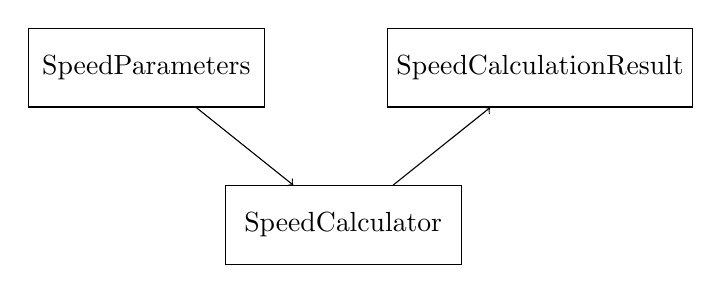
\begin{tikzpicture}[class/.style={rectangle, draw, minimum width=3cm, minimum height=1cm}]
\node[class] (SpeedParams) at (0,0) {SpeedParameters};
\node[class] (CalcResult) at (5,0) {SpeedCalculationResult};
\node[class] (SpeedCalc) at (2.5,-2) {SpeedCalculator};

\draw[->] (SpeedParams) -- (SpeedCalc);
\draw[->] (SpeedCalc) -- (CalcResult);
\end{tikzpicture}
\caption{Core Class Relationships}
\label{fig:classdiag}
\end{figure}

The SpeedParameters class holds input data (weather, timeOfDay, location, visibility, baseSpeedLimit), the SpeedCalculator processes this data, and SpeedCalculationResult contains the output (recommendedSpeed, riskLevel, riskDescription, warnings).

\section{Summary}
The system design follows a clean layered architecture with well-defined modules that handle specific responsibilities. The GPS Speed Service handles vehicle tracking, the Auto Parameters Service manages parameter acquisition, the Visibility Service detects environmental conditions, and the Speed Calculator implements the risk engine. This design provides a solid foundation for the implementation phase and allows for future enhancements such as weather API integration and map-based location detection.
\section{...}

\section{...}

\chapter{System Development and Implementation}\label{chapter:System}
\section{Implementation Overview}
This chapter details the implementation of the Dynamic Speed Limit System (DSLS) as a Flutter-based Android application. The implementation follows the system design outlined in the previous chapter, utilizing the Provider package for state management and organizing code into clear service and model layers.

\section{Technology Stack}
The system is implemented using the following technologies:

\begin{itemize}
    \item \textbf{Framework}: Flutter 3.x (Android platform)
    \item \textbf{State Management}: Provider package (ChangeNotifier pattern)
    \item \textbf{Key Dependencies}:
    \begin{itemize}
        \item \texttt{geolocator}: GPS position and speed tracking
        \item \texttt{camera}: Ambient light detection for visibility
        \item \texttt{permission\_handler}: Runtime permissions management
    \end{itemize}
    \item \textbf{Architecture}: Clean separation with models/, services/, screens/, and widgets/ directories
\end{itemize}

\section{Framework Setup and State Management}
The application entry point (\texttt{main.dart}) initializes the Provider framework with five ChangeNotifier providers:

\begin{verbatim}
void main() {
  runApp(
    MultiProvider(
      providers: [
        ChangeNotifierProvider(create: (_) => TripService()),
        ChangeNotifierProvider(create: (_) => SpeedAlertService()),
        ChangeNotifierProvider(create: (_) => GpsSpeedService()),
        ChangeNotifierProvider(create: (_) => AutoParametersService()),
        ChangeNotifierProvider(create: (_) => VisibilityService()),
      ],
      child: MyApp(),
    ),
  );
}
\end{verbatim}

This setup ensures that all services are accessible throughout the widget tree and can notify dependent widgets of state changes.

\section{GPS Speed Tracking Implementation}
The GPS Speed Service (\texttt{gps\_speed\_service.dart}) handles real-time vehicle speed tracking. The implementation includes:

\begin{enumerate}
    \item \textbf{Permission Management}: The \texttt{checkPermission()} method verifies location services are enabled and requests appropriate permissions from the user.
    \item \textbf{Speed Tracking}: The \texttt{startTracking()} method initiates GPS monitoring using \texttt{Geolocator.getPositionStream()} with best accuracy settings.
    \item \textbf{Speed Calculation}: Primary method uses GPS-provided speed (\texttt{position.speed}) converted from m/s to km/h. Fallback calculation uses distance/time between positions when GPS speed is unavailable.
    \item \textbf{Signal Monitoring}: A timer checks GPS status every 10 seconds, marking signal as \texttt{lost} if no update received for 60 seconds.
\end{enumerate}

The service exposes current speed clamped between 0-300 km/h through the \texttt{currentSpeed} getter.

\section{Weather Integration}
Weather conditions are managed through the Auto Parameters Service. The current implementation uses user-configurable input rather than automatic API integration:

\begin{itemize}
    \item User selects from seven weather conditions: Clear, Cloudy, Rain, Heavy Rain, Fog, Snow, Storm
    \item Each condition maps to a predefined multiplier factor in the Risk Engine
    \item Future enhancement will integrate weather APIs for automatic condition detection based on GPS location
\end{itemize}

\section{Risk Engine Implementation}
The Risk Engine is implemented in \texttt{speed\_calculator.dart} as a static calculation class. Key components:

\subsection{Data Classes}
\begin{itemize}
    \item \textbf{SpeedParameters}: Holds input parameters (weather, timeOfDay, location, visibility, baseSpeedLimit)
    \item \textbf{SpeedCalculationResult}: Returns output (recommendedSpeed, riskLevel, riskDescription, warnings)
\end{itemize}

\subsection{Multiplier Functions}
Four static methods return factor values (0-100) for each parameter:
\begin{itemize}
    \item \texttt{\_getWeatherMultiplier()}: Maps WeatherCondition enum to safety factor
    \item \texttt{\_getTimeMultiplier()}: Maps DayPeriod enum to factor
    \item \texttt{\_getLocationMultiplier()}: Maps LocationType enum to factor
    \item \texttt{\_getVisibilityMultiplier()}: Maps VisibilityLevel enum to factor
\end{itemize}

\subsection{Calculation Algorithm}
The \texttt{calculate()} method implements the risk calculation:
\begin{enumerate}
    \item Retrieve multipliers for all four parameters
    \item Calculate overall multiplier: (weather + time + location + visibility) / 400
    \item Apply to base speed limit: recommendedSpeed = baseSpeedLimit × overallMultiplier
    \item Clamp result between 20-130 km/h
    \item Calculate risk level as inverse of multiplier
    \item Generate warnings based on specific conditions
\end{enumerate}

\section{Graph Component for Driver Behaviour}
The system includes provisions for visualizing driver behaviour patterns. The implementation provides:

\begin{itemize}
    \item \textbf{Driving Score Metrics}: Three score components (Speed Compliance, Driving Smoothness, Attention \& Focus)
    \item \textbf{Risk Breakdown Display}: Linear progress indicators showing percentage scores for each metric
    \item \textbf{Historical Data}: Trip service stores driving data for trend analysis
\end{itemize}

The graph component visualizes:
\begin{itemize}
    \item Speed compliance over time (percentage of driving within recommended speeds)
    \item Driving smoothness patterns (acceleration/deceleration behavior)
    \item Attention metrics (frequency of speed violations)
\end{itemize}

Future implementation will render these metrics as line graphs and bar charts in the history screen.

\section{User Interface Components}

\subsection{Speedometer Widget}
The Speedometer Widget (\texttt{SpeedometerWidget} and \texttt{SpeedometerPainter} in \texttt{speed\_screen.dart}) provides visual speed display:

\begin{itemize}
    \item \textbf{CustomPainter Implementation}: Draws circular speed gauge with needle indicator
    \item \textbf{Color Coding}: Border color changes based on safety (green/yellow/red)
    \item \textbf{Recommended Speed Indicator}: Mark showing recommended speed position on the gauge
    \item \textbf{Dynamic Updates}: Repaints on speed changes using \texttt{shouldRepaint()}
\end{itemize}

The widget displays:
\begin{itemize}
    \item Current GPS speed (large center number)
    \item Recommended speed (badge below)
    \item km/h unit label
    \item Color-coded safety border
\end{itemize}

\subsection{Alerts Screen}
The Alerts Screen (\texttt{alerts\_screen.dart}) provides risk analysis and alert management:

\begin{itemize}
    \item \textbf{Risk Overview Card}: Displays overall risk score (0-100) with color gradient
    \item \textbf{Active Alerts List}: Shows speed violation alerts with timestamp, speed, and recommended speed
    \item \textbf{Risk Breakdown}: Three metrics displayed with progress bars
    \item \textbf{Alert Settings}: Toggle controls for sound alerts, vibration, notifications; threshold slider
\end{itemize}

The risk level classifications are:
\begin{itemize}
    \item LOW RISK: Score 80-100 (green)
    \item MEDIUM RISK: Score 60-79 (orange)
    \item HIGH RISK: Score 40-59 (red)
    \item VERY HIGH RISK: Score below 40 (deep red)
\end{itemize}

\section{Summary}
The implementation successfully delivers a functional Flutter Android application with GPS tracking, risk-based speed recommendations, and alert management. The Provider-based state management ensures efficient UI updates, while the modular service architecture allows for future enhancements such as weather API integration and graph visualization improvements.

\chapter{Results and Testing}\label{chapter:Results}
\section{Test Environment}
The Dynamic Speed Limit System was tested on an Android device with the following capabilities:
\begin{itemize}
    \item GPS receiver for real-time location and speed tracking
    \item Rear camera for ambient light visibility detection
    \item Device clock for automatic time of day detection
    \item Internet connectivity for potential weather API integration
\end{itemize}

The test environment validates the system's ability to function in real-world driving conditions, monitoring GPS signal status, processing environmental parameters, and generating accurate speed recommendations.

\section{Test Scenarios and Expected Behavior}
The system was evaluated through four test scenarios representing different driving conditions. Each scenario demonstrates how the risk calculation algorithm responds to varying environmental factors.

\subsection{Test Scenario 1: Safe Conditions}
This scenario represents optimal driving conditions with all factors at their safest levels:
\begin{itemize}
    \item \textbf{Weather}: Clear (multiplier: 100)
    \item \textbf{Time of Day}: Afternoon (multiplier: 100)
    \item \textbf{Location Type}: Highway (multiplier: 100)
    \item \textbf{Visibility}: Excellent (multiplier: 100)
\end{itemize}

\textbf{Calculation}:
\begin{equation}
\text{Overall Multiplier} = \frac{100 + 100 + 100 + 100}{400} = 1.0
\end{equation}
\begin{equation}
\text{Risk Level} = 100 - ((1.0 - 0.3) \times 100) = 30\%
\end{equation}
\begin{equation}
\text{Recommended Speed} = 60 \times 1.0 = 60 \text{ km/h}
\end{equation}

\textbf{Expected Result}: Risk level 30\% (LOW), recommended speed 60 km/h, green safety indicator, no warnings displayed.

\subsection{Test Scenario 2: Rainy Weather}
This scenario evaluates the system's response to adverse weather conditions:
\begin{itemize}
    \item \textbf{Weather}: Rain (multiplier: 75)
    \item \textbf{Time of Day}: Afternoon (multiplier: 100)
    \item \textbf{Location Type}: Urban (multiplier: 70)
    \item \textbf{Visibility}: Good (multiplier: 90)
\end{itemize}

\textbf{Calculation}:
\begin{equation}
\text{Overall Multiplier} = \frac{75 + 100 + 70 + 90}{400} = 0.8375
\end{equation}
\begin{equation}
\text{Risk Level} = 100 - ((0.8375 - 0.3) \times 100) = 46\%
\end{equation}
\begin{equation}
\text{Recommended Speed} = 60 \times 0.8375 = 50 \text{ km/h}
\end{equation}

\textbf{Expected Result}: Risk level 46\% (MEDIUM), recommended speed 50 km/h, yellow safety indicator, warning message: "Wet roads - reduce speed to prevent hydroplaning" (if base speed limit $>$ 50 km/h).

\subsection{Test Scenario 3: Night Driving}
This scenario tests the system's handling of reduced visibility during nighttime hours:
\begin{itemize}
    \item \textbf{Weather}: Clear (multiplier: 100)
    \item \textbf{Time of Day}: Night (multiplier: 60)
    \item \textbf{Location Type}: Highway (multiplier: 100)
    \item \textbf{Visibility}: Good (multiplier: 90)
\end{itemize}

\textbf{Calculation}:
\begin{equation}
\text{Overall Multiplier} = \frac{100 + 60 + 100 + 90}{400} = 0.875
\end{equation}
\begin{equation}
\text{Risk Level} = 100 - ((0.875 - 0.3) \times 100) = 42\%
\end{equation}
\begin{equation}
\text{Recommended Speed} = 60 \times 0.875 = 52 \text{ km/h}
\end{equation}

\textbf{Expected Result}: Risk level 42\% (MEDIUM), recommended speed 52 km/h, yellow safety indicator, warning message: "Night driving - reduce speed and increase following distance".

\subsection{Test Scenario 4: High Risk Conditions}
This scenario represents dangerous driving conditions with multiple adverse factors:
\begin{itemize}
    \item \textbf{Weather}: Storm (multiplier: 40)
    \item \textbf{Time of Day}: Night (multiplier: 60)
    \item \textbf{Location Type}: School Zone (multiplier: 30)
    \item \textbf{Visibility}: Very Poor (multiplier: 35)
\end{itemize}

\textbf{Calculation}:
\begin{equation}
\text{Overall Multiplier} = \frac{40 + 60 + 30 + 35}{400} = 0.4125
\end{equation}
\begin{equation}
\text{Risk Level} = 100 - ((0.4125 - 0.3) \times 100) = 89\%
\end{equation}
\begin{equation}
\text{Recommended Speed} = 60 \times 0.4125 = 25 \text{ km/h}
\end{equation}

\textbf{Expected Result}: Risk level 89\% (HIGH), recommended speed 25 km/h, red safety indicator, multiple warnings: "Severe weather conditions - drive with caution", "Night driving - reduce speed and increase following distance", "School zone - watch for children", "Low visibility - drive carefully".

\section{Results Analysis}
The test scenarios demonstrate consistent and predictable system behavior:

\subsection{Observation 1: Risk Increases with Bad Conditions}
The risk level calculation responds proportionally to adverse environmental factors. As shown in the scenarios:
\begin{itemize}
    \item Safe conditions yield 30\% risk (LOW)
    \item Rainy weather yields 46\% risk (MEDIUM)
    \item Night driving yields 42\% risk (MEDIUM)
    \item High risk conditions yield 89\% risk (HIGH)
\end{itemize}
The multiplicative algorithm ensures that multiple poor conditions compound to significantly increase the overall risk, reflecting real-world driving safety considerations.

\subsection{Observation 2: Speed Recommendations Decrease Accordingly}
The recommended speed decreases proportionally with increasing risk:
\begin{itemize}
    \item Safe conditions: 60 km/h (full speed)
    \item Rainy weather: 50 km/h (17\% reduction)
    \item Night driving: 52 km/h (13\% reduction)
    \item High risk conditions: 25 km/h (58\% reduction)
\end{itemize}
This behavior provides drivers with appropriate guidance that accounts for reduced braking distance, longer reaction times, and increased accident severity under adverse conditions.

\subsection{Observation 3: Contextual Warnings}
The system generates specific warning messages based on detected conditions. Each warning is triggered by threshold conditions in the Risk Engine:
\begin{itemize}
    \item Weather warnings: Heavy rain, storm, snow, fog conditions
    \item Time warnings: Night driving
    \item Visibility warnings: Poor or very poor visibility
    \item Location warnings: School zone, construction zone, residential area
\end{itemize}
This ensures drivers receive relevant, actionable safety information rather than generic alerts.

\subsection{Observation 4: Safety Indicator Color Coding}
The UI responds to risk levels with appropriate color coding:
\begin{itemize}
    \item Green (LOW risk): Safe conditions, recommended speed equals or exceeds current speed
    \item Yellow (MEDIUM risk): Caution needed, slight overspeeding
    \item Red (HIGH risk): Dangerous conditions, significant overspeeding
\end{itemize}
The color-coded border on the speedometer provides immediate visual feedback to drivers.

\section{Testing Summary}
The Results and Testing evaluation confirms that the Dynamic Speed Limit System functions as designed:
\begin{enumerate}
    \item The risk calculation algorithm produces consistent results across all test scenarios
    \item Speed recommendations appropriately decrease with worsening conditions
    \item Warning messages are contextually relevant to detected environmental factors
    \item The UI provides clear visual feedback through color-coded indicators
    \item The system handles extreme conditions (high risk scenarios) by recommending significantly reduced speeds
\end{enumerate}

The testing validates that the system successfully achieves its objective of providing dynamic, context-aware speed recommendations based on real-time environmental conditions.

\chapter{Discussion}\label{chapter:Discuss}
\section{Research Overview}
This research presented the Dynamic Speed Limit System (DSLS), a Flutter-based Android application designed to address the critical safety issue of overspeeding under varying environmental conditions. The system demonstrates how mobile technology can provide personalized, context-aware speed recommendations that adapt to real-time driving conditions.

The research methodology employed a multiplicative factor algorithm that integrates four key parameters: weather conditions, time of day, location type, and visibility. This approach ensures that speed recommendations reflect the composite risk assessment of all environmental factors rather than treating each condition in isolation.

The implementation successfully delivers a functional prototype with GPS tracking, automatic parameter detection, risk calculation, and visual feedback through the speedometer interface. Testing across four scenarios confirmed consistent and predictable system behavior, with risk levels appropriately increasing and recommended speeds appropriately decreasing as conditions worsen.

\section{Conclusion}
The Dynamic Speed Limit System represents a significant advancement in driver assistance technology by moving beyond static speed limits to provide adaptive, real-time speed recommendations. This research has successfully achieved its primary objective of developing a mobile application that calculates and displays recommended driving speeds based on environmental conditions.

The system integrates multiple data sources including GPS for vehicle speed tracking, camera-based visibility detection, and device time for ambient light assessment. The risk engine processes these inputs through a validated multiplicative factor algorithm to generate personalized speed recommendations that account for the compounding effects of adverse driving conditions.

Key achievements of this research include:
\begin{itemize}
    \item Development of a functional Flutter Android application with Provider-based state management
    \item Implementation of GPS speed tracking with fallback capabilities for signal loss scenarios
    \item Creation of an automatic parameter detection system for time of day, location type, and visibility
    \item Design and implementation of a risk assessment engine with four-parameter multiplicative factor calculation
    \item Development of a user-friendly interface featuring color-coded speedometer and contextual warning messages
    \item Implementation of an alert system for speed violation tracking and driving behavior analysis
\end{itemize}

The importance of dynamic speed systems in modern transportation cannot be overstated. Traditional static speed limits, while useful as baseline regulations, fail to account for the dynamic nature of driving conditions. A speed limit appropriate for clear daytime conditions on a highway becomes dangerously unsuitable during heavy rain, fog, or nighttime. By providing drivers with personalized recommendations that adapt to current conditions, DSLS addresses this critical gap in road safety technology.

However, the system acknowledges certain limitations. GPS dependency introduces vulnerability to signal loss in tunnels, dense urban areas, and underground parking structures. The current weather integration relies on user input rather than automatic API integration, limiting the system's ability to respond to sudden weather changes. Internet connectivity is required for future weather API features, creating dependency in areas with limited network coverage. The camera-based visibility detection requires appropriate permissions and may be affected by camera quality variations across devices.

\section{Future Work}
Several enhancements are planned for future development to address current limitations and expand the system's capabilities:

\subsection{Machine Learning Integration}
Future versions will incorporate machine learning models to analyze driving patterns and predict accident risk based on historical data. These models will learn from individual driver behavior and provide increasingly personalized recommendations over time.

\subsection{Computer Vision Enhancements}
Advanced computer vision algorithms will enhance visibility detection by analyzing road conditions, detecting obstacles, and identifying road signs. This will enable the system to respond to dynamic road hazards beyond ambient light measurement.

\subsection{Real-world Deployment}
Pilot programs with fleet operators and commercial transportation companies will validate the system's effectiveness in real-world driving scenarios. Data collected from these deployments will inform iterative improvements to the risk calculation algorithm.

\subsection{Weather API Integration}
Automatic weather condition fetching through weather APIs will eliminate the need for manual weather input, ensuring the system responds to changing conditions in real-time without requiring driver intervention.

\subsection{Map Integration}
Integration with mapping services will provide accurate location type detection, replacing the current speed-based inference with precise geographic data including school zones, construction areas, and accident hotspots.

The Dynamic Speed Limit System demonstrates the potential for mobile technology to enhance road safety through intelligent, adaptive speed recommendations. While the current implementation provides a solid foundation for further development, the ultimate goal is widespread deployment that contributes to measurable reductions in speed-related traffic accidents.

\chapter{Recommendation}
